\section{问题一:烟幕干扰弹的投放策略}

\subsection{数学建模}

基于上述假设和符号定义,我们构建了运动学与几何遮蔽模型。

\textbf{运动轨迹模型:}导弹、无人机、烟幕云团中心的运动轨迹分别由以下方程描述。导弹位置为:
\[
R_M(t) = P_{M1} + v_M \cdot \mathbf{u}_M \cdot t
\]

无人机位置为:
\[
R_{FY1}(t) = P_{FY1} + v_D \cdot \mathbf{u}_{FY1} \cdot t
\]

烟幕弹投放时刻与位置为:$t_{rel} = t_{delay}$,$P_{rel} = R_{FY1}(t_{rel})$。烟幕弹起爆时刻与位置为:$t_{det} = t_{rel} + t_{det\_delay}$,起爆点 $P_{det}$ 的坐标由 $P_{rel}$、无人机速度 $v_D$ 和自由落体公式确定。烟幕云团中心位置($t \ge t_{det}$)为:
\[
C(t) = P_{det} - (0, 0, v_{cloud}(t - t_{det}))
\]

\textbf{几何遮蔽判定模型:}在任意时刻 $t$($t \ge t_{det}$),对于真目标圆柱体表面的任意一点 $Q$,连接导弹位置 $R_M(t)$ 与 $Q$ 的视线线段为:
\[
\ell(s) = R_M(t) + s(Q - R_M(t)), \quad s \in [0, 1]
\]

该视线被遮蔽的条件是,线段 $\ell(s)$ 与以 $C(t)$ 为中心、$r_{cloud}$ 为半径的球体相交。这等价于线段到球心的最小距离不大于球体半径:
\[
\min_{s \in [0,1]} \|\ell(s) - C(t)\| \le r_{cloud}
\]

真目标在时刻 $t$ 被完全遮蔽的充要条件是,对于圆柱表面上的所有点 $Q$,上述不等式均成立。

\subsection{计算结果与分析}

为求解该模型,我们采用“粗略扫描-精确求解”的数值算法。首先在烟幕云团的有效时间域内进行离散时间点扫描,初步定位遮蔽区间;然后利用二分法在区间边界进行高精度迭代,最终得到精确的遮蔽起止时刻。计算结果如表~\ref{tab:q1_results}所示。

\begin{table}[htbp]
\centering
\caption{问题一计算结果}
\label{tab:q1_results}
\begin{tabular}{lc}
\toprule
\textbf{参数} & \textbf{数值} \\
\midrule
烟幕弹投放时刻 & 1.5 s \\
烟幕弹起爆时刻 & 5.1 s \\
有效遮蔽开始时刻 & 8.056443 s \\
有效遮蔽结束时刻 & 9.448088 s \\
有效遮蔽总时长 & 1.391645 s \\
\bottomrule
\end{tabular}
\end{table}

表~\ref{tab:q1_results}显示了关键时间节点的计算结果。烟幕弹在1.5s投放、5.1s起爆后,有效遮蔽时间段为8.056443s至9.448088s,总时长1.391645秒。

图~\ref{fig:q1_visualization}直观展示了遮蔽过程的动态特征。上图的遮蔽状态曲线清晰标识了有效遮蔽时间段,下图的距离变化曲线显示当烟幕云团中心到导弹-目标视线距离小于10.00m时实现遮蔽,距离曲线呈现先减小后增大的趋势,反映了导弹与烟幕云团的相对运动关系。

\begin{figure}[htbp]
\centering
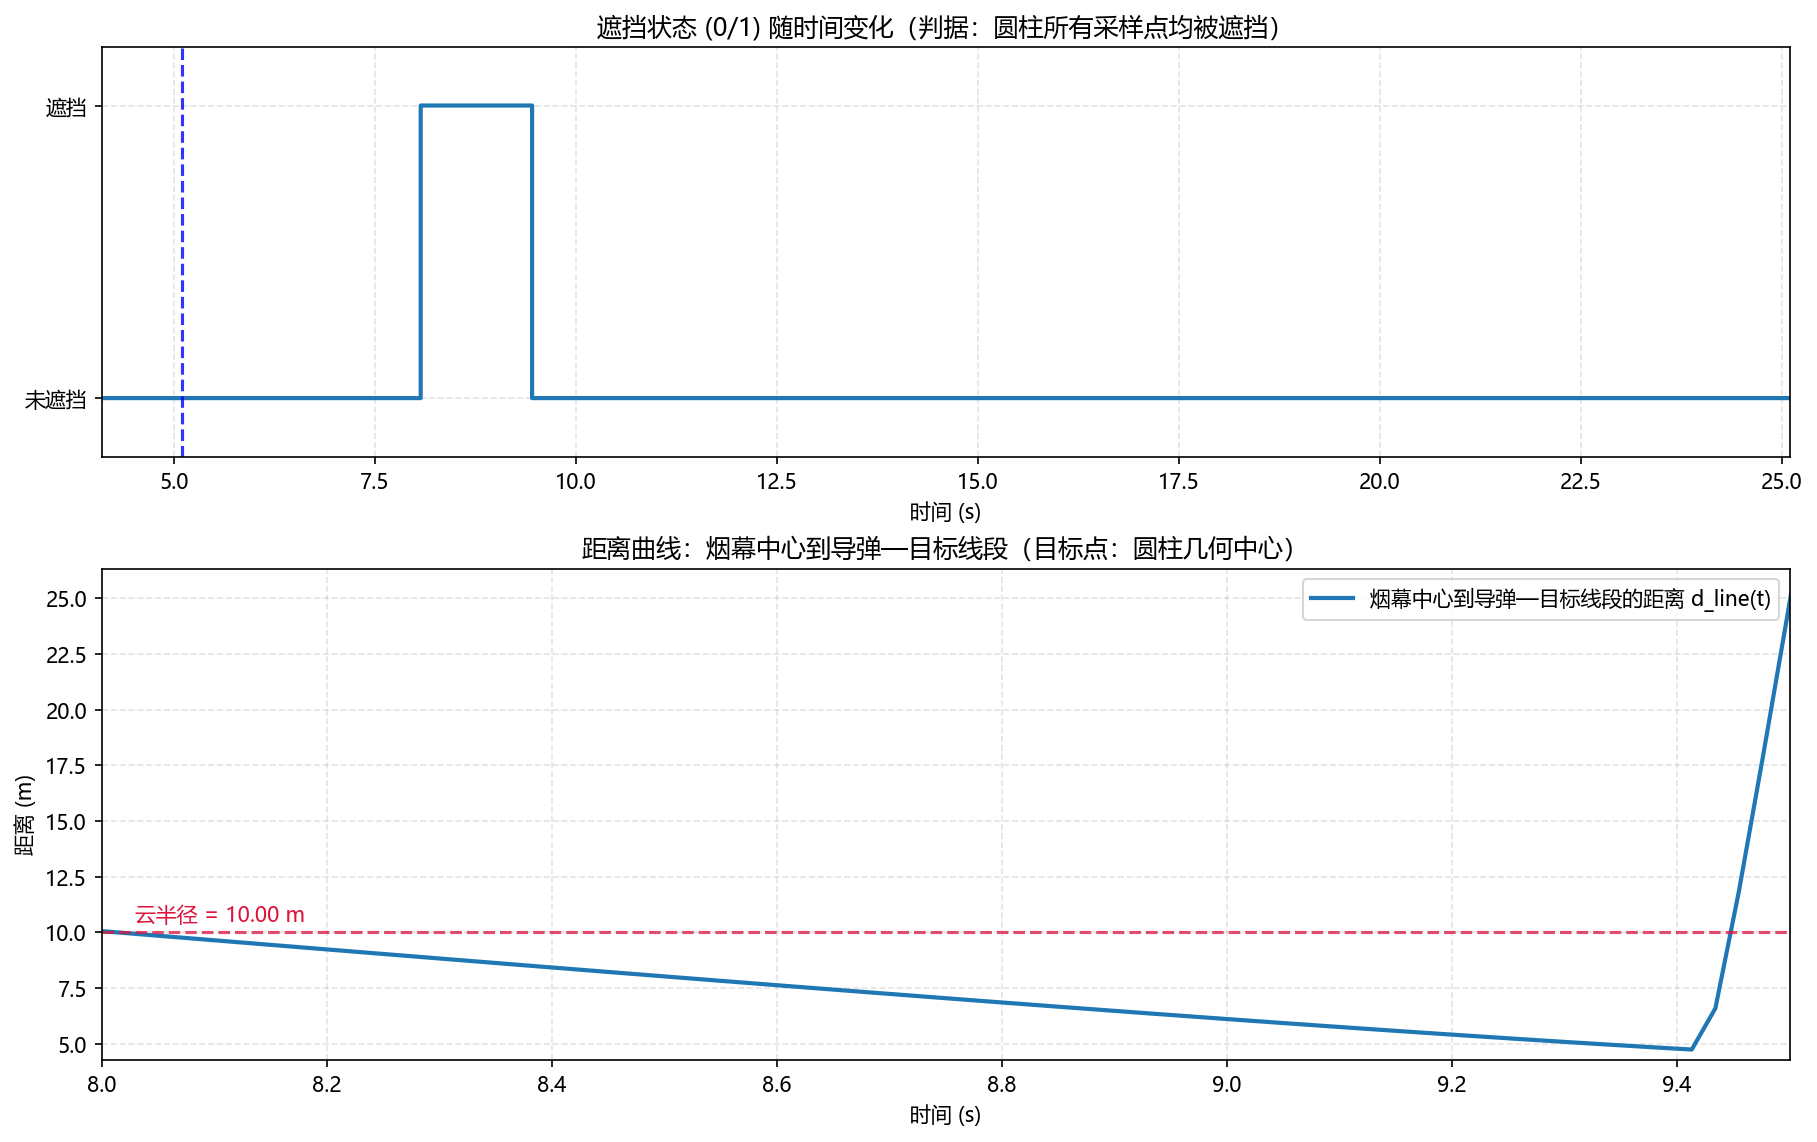
\includegraphics[width=\textwidth]{figures/A_1_1.png}
\caption{问题一遮蔽效果可视化分析}
\label{fig:q1_visualization}
\end{figure}

\subsection{第二种解法:基于光线追踪与符号计算的几何分析方法}

为了验证第一种解法的准确性并提供更直观的几何理解,我们开发了基于光线追踪和符号计算的第二种解法。该方法从光学投影的角度重新审视遮蔽问题,通过分析导弹视线在目标平面上的投影阴影来判定遮蔽效果。

\textbf{第二种解法符号说明:}为了清晰描述第二种解法的数学模型,我们补充定义如表~\ref{tab:symbols_q1_method2}所示的符号。

\begin{table}[htbp]
\centering
\caption{第二种解法补充符号说明}
\label{tab:symbols_q1_method2}
\begin{tabular}{cc}
\toprule
\textbf{符号} & \textbf{说明} \\
\midrule
$\mathbf{P}_{missile}$ & 导弹在时刻$t$的位置 \\
$\mathbf{P}_{plane}$ & yOz平面上的任意点$(0, y, z)$ \\
$\mathbf{r}(t)$ & 从导弹到平面点的射线方程 \\
$\mathbf{P}_1(t)$ & 导弹位置的符号表示 \\
$\mathbf{P}_2$ & 真目标圆柱体下底面中心$(0, 200, 0)$ \\
$\mathbf{P}_3$ & 真目标圆柱体上底面中心$(0, 200, 10)$ \\
$\mathbf{Q}(t)$ & 烟幕云团中心位置 \\
$d_1(t)$ & 云团中心到导弹-下底面中心连线的距离 \\
$d_2(t)$ & 云团中心到导弹-上底面中心连线的距离 \\
\bottomrule
\end{tabular}
\end{table}

\textbf{光线追踪投影模型:}将导弹视作点光源,烟幕云团视作球形遮挡物,真目标所在的yOz平面视作投影屏幕。通过光线追踪算法计算烟幕云团在yOz平面上形成的阴影区域。对于平面上的每个点$(0, y, z)$,从导弹位置发出射线,判断该射线是否与烟幕云团球体相交:
\[
\text{射线方程:} \mathbf{r}(t) = \mathbf{P}_{missile} + t(\mathbf{P}_{plane} - \mathbf{P}_{missile})
\]
\[
\text{球体方程:} \|\mathbf{r}(t) - \mathbf{C}\|^2 = r_{cloud}^2
\]
其中$\mathbf{C}$为云团中心,$r_{cloud}$为云团半径。通过求解二次方程的判别式确定射线与球体的交点,进而确定阴影区域。

\[
d_1(t) = \frac{\|(\mathbf{P}_2 - \mathbf{P}_1) \times (\mathbf{Q} - \mathbf{P}_1)\|}{\|\mathbf{P}_2 - \mathbf{P}_1\|}
\]
\[
d_2(t) = \frac{\|(\mathbf{P}_3 - \mathbf{P}_1) \times (\mathbf{Q} - \mathbf{P}_1)\|}{\|\mathbf{P}_3 - \mathbf{P}_1\|}
\]
当$d_1(t) \leq r_{cloud}$且$d_2(t) \leq r_{cloud}$同时满足时,烟幕云团对导弹观测真目标形成有效遮蔽。

此计算方法得到的有效遮蔽时间段为 [8.0561, 9.4536] 秒,遮蔽总时长为 1.3975 秒,与第一种方法的结果 [8.0564, 9.4481] 秒(总时长 1.3916 秒)高度一致,验证了计算的准确性。图~\ref{fig:q1_method2_visualization}展示了第二种解法的几何分析结果:左图显示了烟幕云团在 yOz 平面上的投影圆与真目标矩形区域的位置关系;右图为三维空间中的光线追踪可视化,展现了导弹视线、烟幕云团、投影阴影以及光线边界的空间关系。第二种解法通过光线追踪可视化提供了更直观的几何理解,投影圆与目标矩形的重叠程度直接反映遮蔽效果强弱,三维视图展现了整个遮蔽过程的空间几何特征,验证了数值计算结果的合理性。

\begin{figure}[htbp]
\centering
\begin{minipage}{0.48\textwidth}
\centering
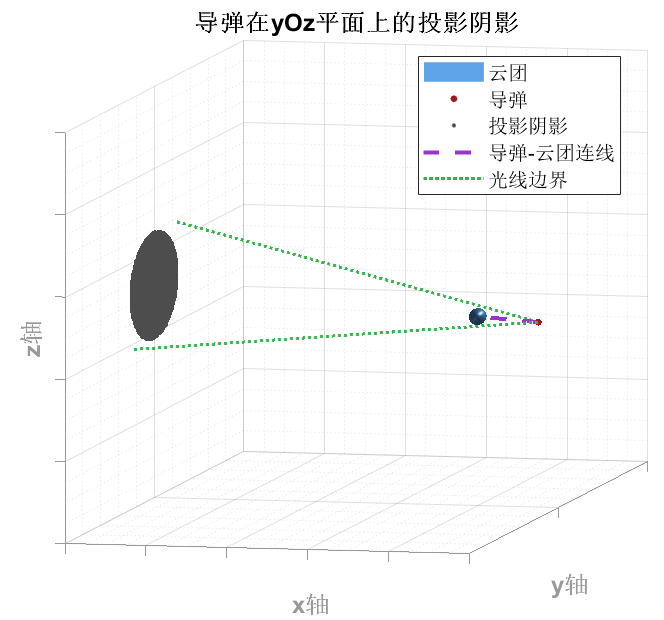
\includegraphics[width=0.8\textwidth]{figures/A_1_2.png}
\end{minipage}
\hfill
\begin{minipage}{0.48\textwidth}
\centering
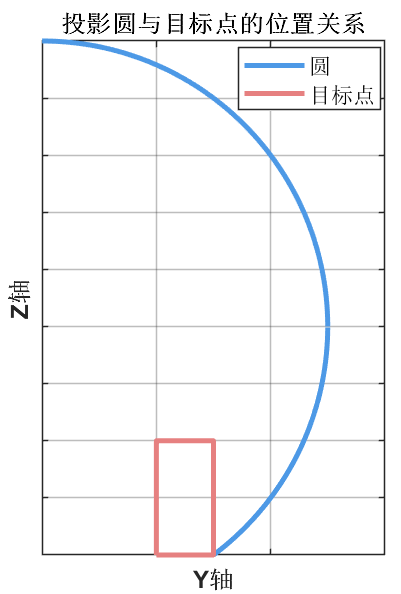
\includegraphics[width=0.8\textwidth]{figures/A_1_3.png}
\end{minipage}
\caption{第二种解法几何分析可视化:(左)投影圆与目标位置关系;(右)三维光线追踪示意图}
\label{fig:q1_method2_visualization}
\end{figure}